\documentclass[letterpaper, 10 pt, conference]{article} 
\usepackage[english]{babel}
\usepackage{amsmath,amssymb,amscd,amsthm} % variety of useful math macros
\usepackage[inner=1.5 cm, outer = 1.5 cm, top=1 cm, bottom = 1.5 cm]{geometry}
\usepackage{subcaption}
%For inserting graphics
\usepackage{graphicx}
\usepackage[dvipsnames]{xcolor}
\usepackage{listings}
\usepackage[utf8]{inputenc}
\usepackage{hyperref}
\usepackage{algpseudocode,algorithm}
%For diagrams
%\usepackage{tikz} 


\newcommand\N{\ensuremath{\mathcal{N}}}		%N for networks
\renewcommand{\P}{\ensuremath{\mathbb{P}}} %P for probability measures
\renewcommand{\iff}{\ensuremath{\Leftrightarrow}} %Shorter \iff 

%\newtheorem{theorem}{Theorem}
\newtheorem{prop}{Proposition}
\newtheorem{lemma}{Lemma}


\title{Pseudo-random number generators}
\author{G. Palafox}


\begin{document}

\maketitle

\begin{abstract}
Various pseudo-random number generators are exhibited and compared. Statistical tests are run to determine their performance. Variations are studied to analyze the sensitivity of the algorithms. 
\end{abstract}

\section{Introduction}
In the present work, different pseudo-random number generators are studied. In particular, methods for generating uniform distributed pseudo-random numbers and normal distributed pseudo-random numbers are studied. Their efficacy is statistically tested with Frosini's uniformity test and Shapiro's Normality test, respectively.Additionally, the sensitivity of some of the methods is tested by varying their input parameters and measuring possible changes in the quality of the output. A time comparison is also carried out to compare the performance of some of the methods. This study was performed with R version 4.0.0 \cite{R} on a Jupyter \cite{jupyter} notebook\footnote{The notebook with the code containing our analysis, as well as this report, can be found in the Github Repository: \url{https://github.com/palafox794/AppliedProbabilityModels/tree/master/Assignment5}}. 

\section{Methods for the uniform distribution}
First, the simplest of the methods is studied: the linear congruential generator (\textsc{LGC}). Parameters are varied to look for differences in its output. Then, the Additive Congruential Random Number Generator is looked at. Frosini's test for uniformity \cite{Blinov_Lemeshko_2014} is performed on data outputted by both algorithms.

\subsection{Linear Congruential Method}
This method outputs a sequence of $n$ numbers uniformly distributed on $(0,1)$.  Pseudo-code for this method is shown in Algorithm \ref{algo:lgc}. It is based on the recurrence relation 
\begin{equation}
X_{n+1} = (a X_n + c) \mod m,
\end{equation}
 where $X_0, a, c$ and $m$ are integers chosen by the user. The algorithm outputs at most $m$ distinct numbers, but the possibility of patterns of length shorter than $m$ occurring exist. Necessary and sufficient conditions for achieving an $m$-length sequence are known \cite{Hull_Dobell_1962}: $a, m$ must be coprime, $a-1$ must be divisible by all prime factors of $m$, and $a-1$ need be divisible by 4 if $m$ is divisible by 4. Figure \ref{fig:unif__lgc} shows an histogram of the output of \textsc{LGC} with a seed of $X_0= 101$, and $a = 1151, c = 27077, m = 2^{32}$. The data in this histogram gives us a $p$-value of 0.38 $>$ 0.05 when Frosini's Uniformity test \cite{Blinov_Lemeshko_2014} is performed on it.
To further study this method, a hundred sequences of length one-thousand were generated, and for each, the $p$-value associated to Frosini's test was computed and stored. This was done twice: first, with parameters $a = 2^{10} + 1, c = 2^{16} + 1, m = 2^{32}$ and then with parameters $a = 2^{10}, c = 2^{16} + 1, m = 2^{32}$. Note the first set of parameters satisfy the aforementioned conditions for maximum length while the second set does not. In particular, $a = 2^{10}, m = 2^{32}$ are not coprime. In the first scenario, the $p$-value was greater than 0.05 in 93 out of 100 times. A boxplot of this $p$-values is shown in Figure \ref{fig:boxplot_pvalues_lgc}. For the second scenario, all hundred $p$-values where significantly less than 0.05. 


 \begin{figure}
	\centering
	\begin{subfigure}[b]{0.45\linewidth}
		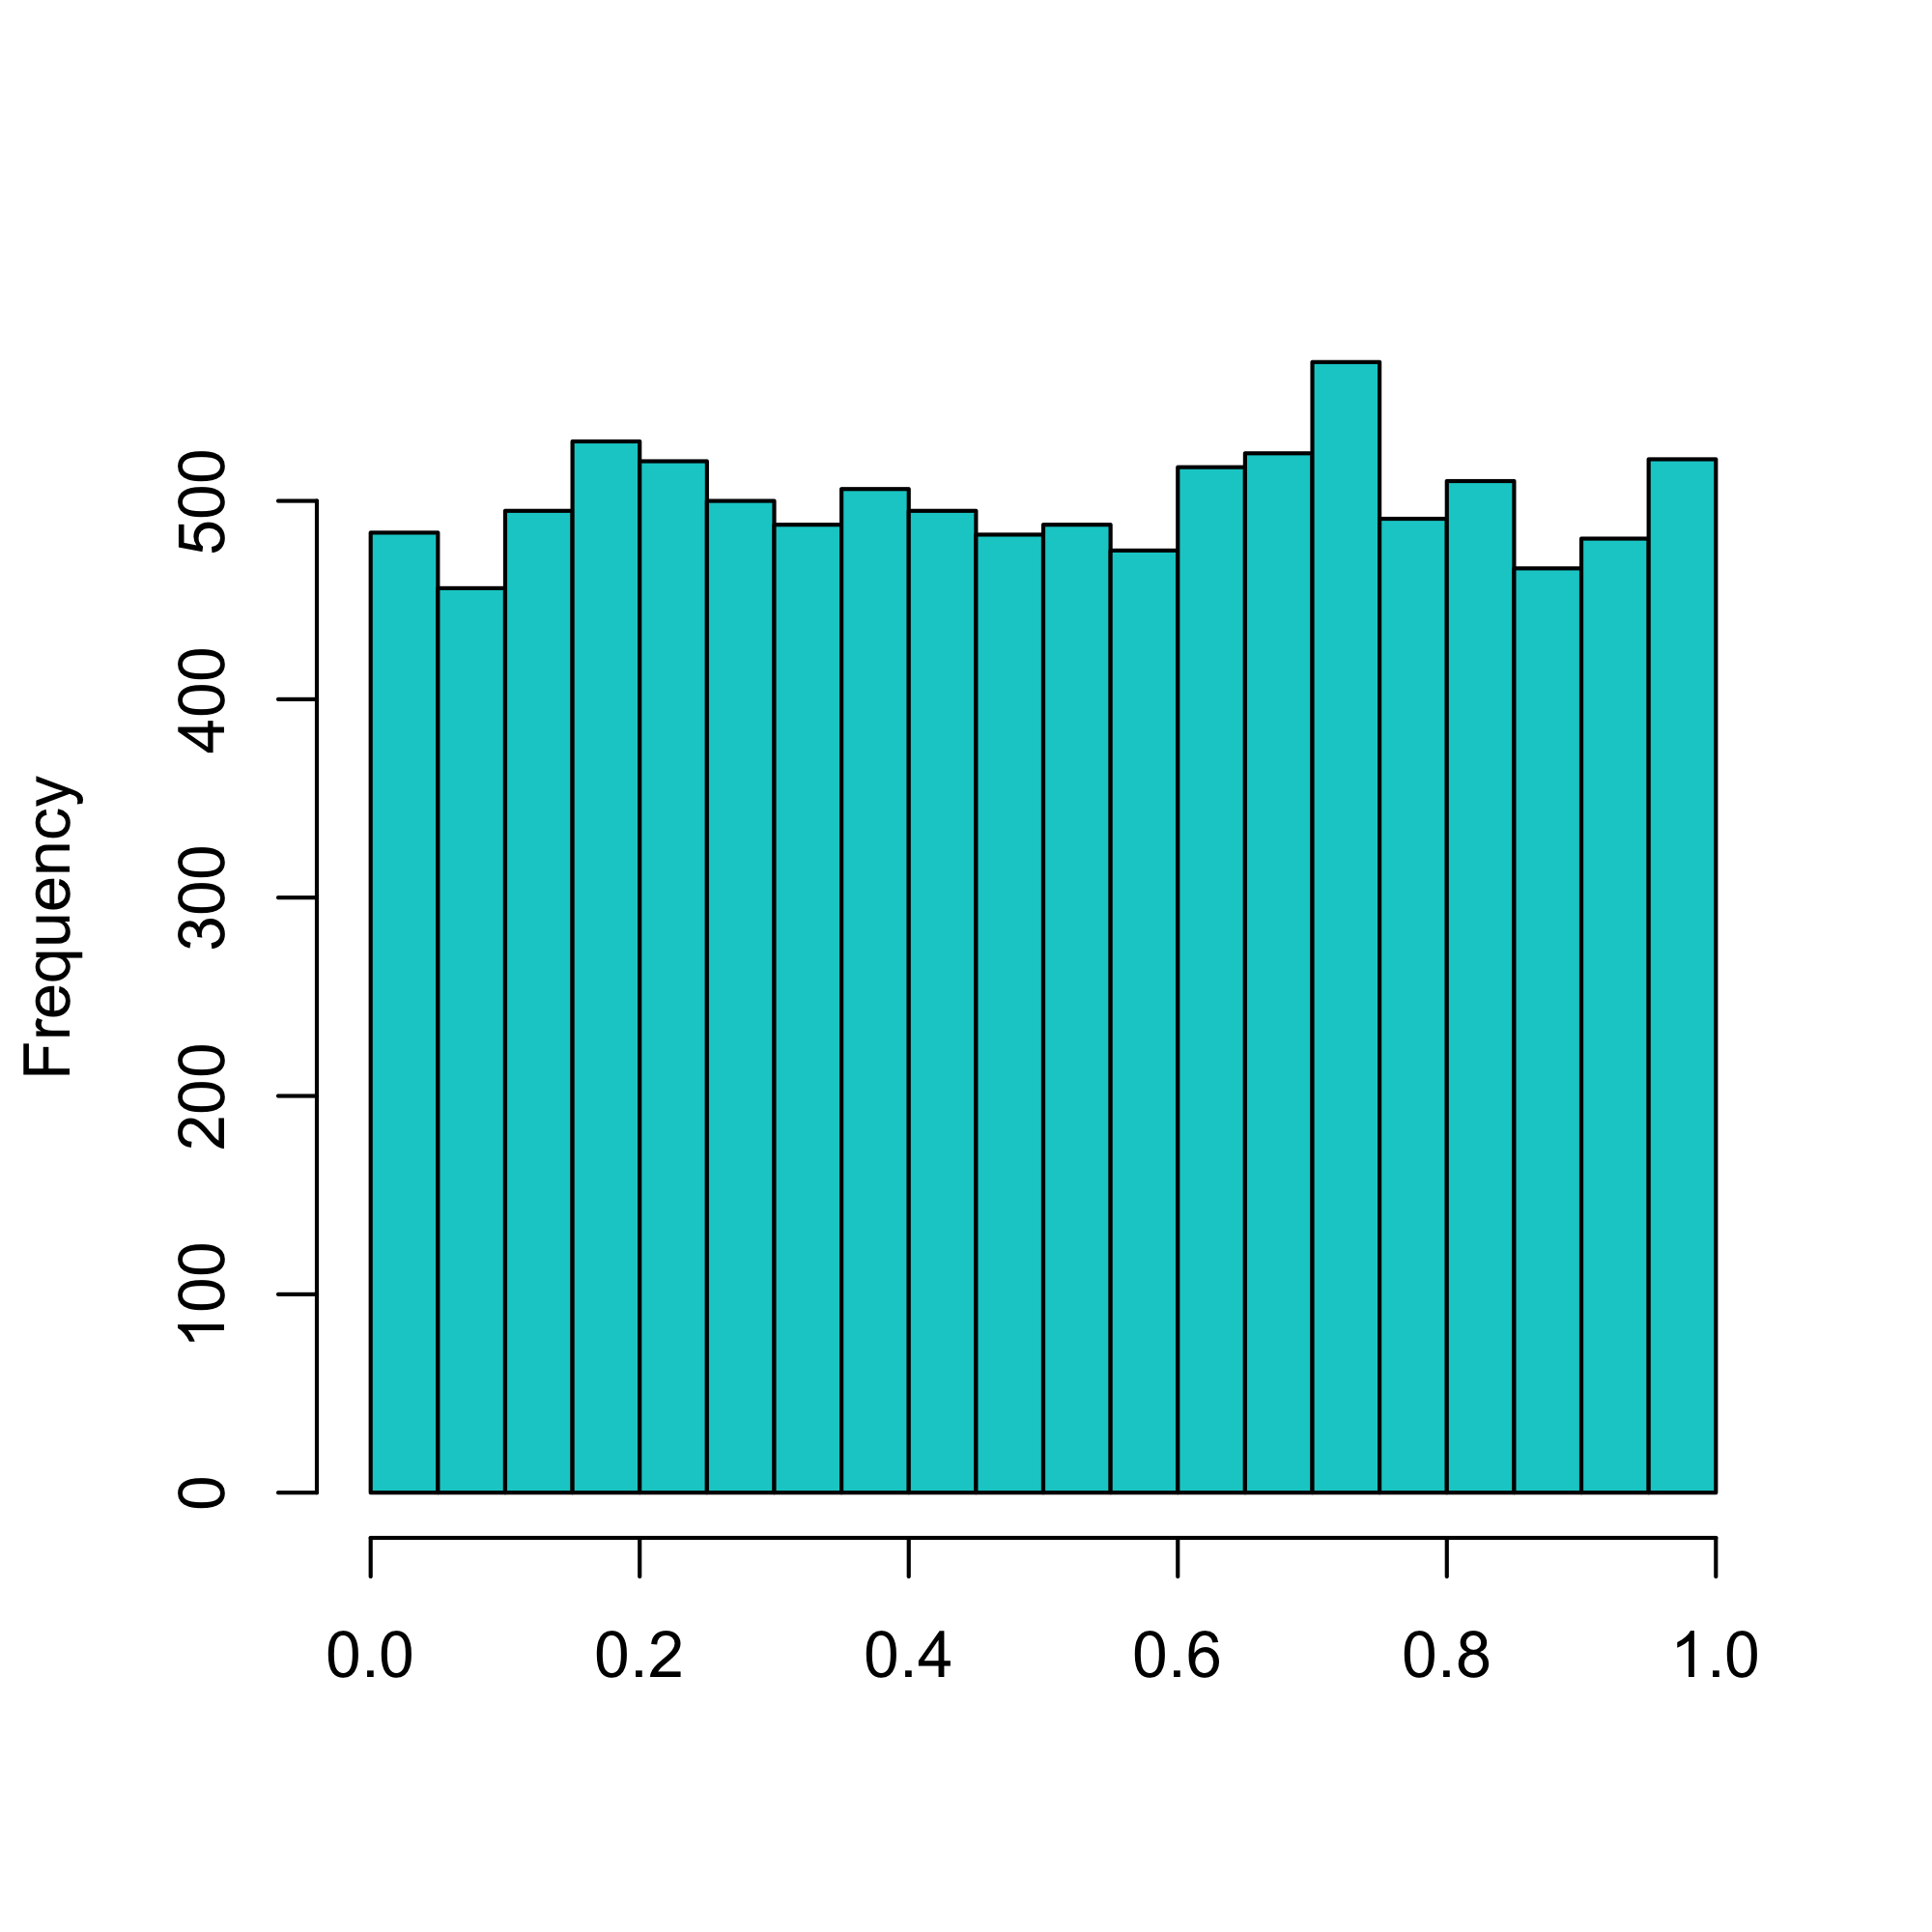
\includegraphics[width=\linewidth]{unif_lgc.png}
		\caption{Histogram of a \textsc{LCG} sample of size ten-thousand, with parameters $a = 1151, c=27077, m=2^{32}$}
		\label{fig:unif__lgc}
	\end{subfigure}
	\hfill
	\begin{subfigure}[b]{0.45\linewidth}
		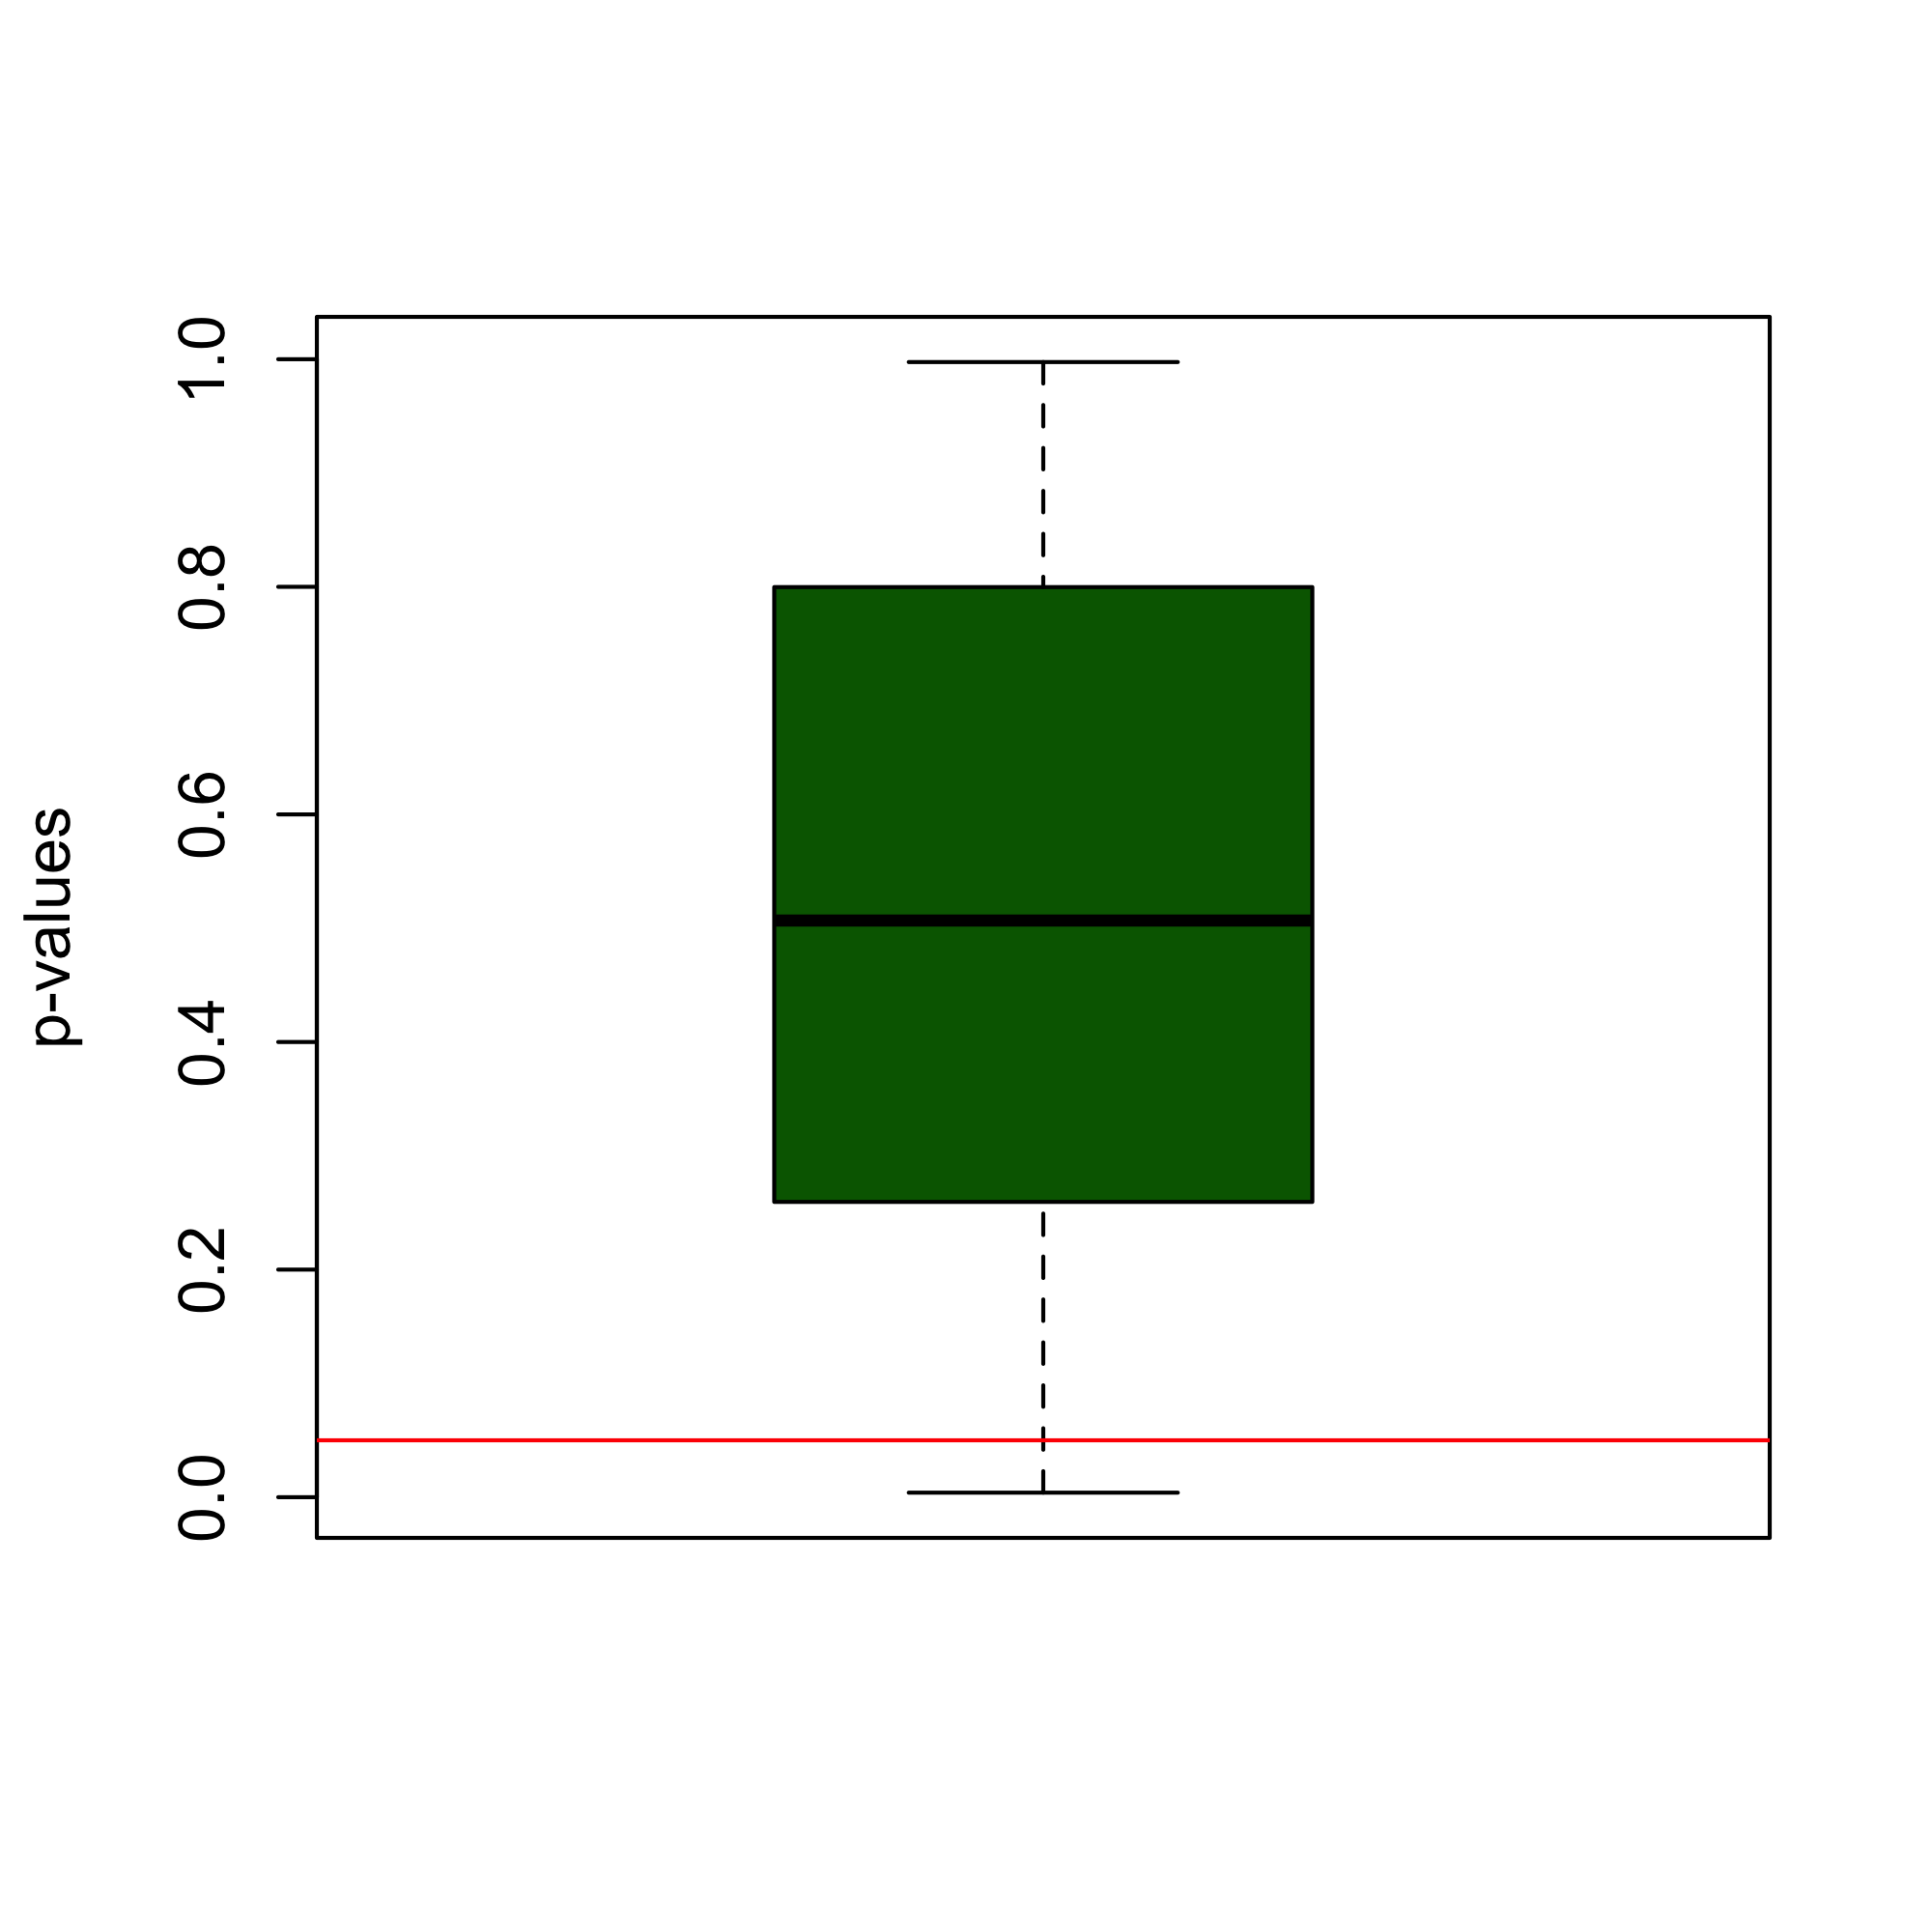
\includegraphics[width=\linewidth]{boxplot_pvalues_lgc}
		\caption{Boxplot of the $p$-values of a hundred \textsc{LCG} samples, with $a = 2^{10} + 1, c = 2^{16} + 1, m = 2^{32}$. Red line is at 0.05}
		\label{fig:boxplot_pvalues_lgc}
	\end{subfigure}
	\caption{Linear congruential generator.} 
	\label{fig:lgc}
\end{figure}

\begin{algorithm}
	\caption{Linear Congruential Generator}
	\begin{flushleft}
		\textbf{Input: } Positive integers \texttt{n, a, c, m, seed}.
		\\ \textbf{Output: } Array of \texttt{n} numbers with $\mathrm{Unif}$(0,1) distribution.
	\end{flushleft}
	
	\begin{algorithmic}[1]
		\State Make empty numeric vector \texttt{numbers}
		\State Make \texttt{x} $=$ \texttt{seed}
		\While{length(\texttt{numbers}) $<$ \texttt{n}}
			\State Make \texttt{x = (a*x + c) mod m}
			\State Append \texttt{x/(m-1)} to \texttt{numbers}
		\EndWhile
		\State \Return \texttt{numbers}
	\end{algorithmic}
	\label{algo:lgc}
\end{algorithm}

\subsection{Additive Congruential Random Number Generator}
Similar as the \textsc{LGC}, the Additive Congruential Random Number Generator (\textsc{ACORN}) \cite{Wikramaratna_1989}  is a method based on modular arithmetic and generates $n$ uniformly distributed pseudo-random numbers. It starts with $k$ initial values $Y_{0}^{m}, m = 1, 2, \dots, k$ all being less than a modulus $M$. With these, the following are defined:
\begin{align}
Y_{n}^{0} &= Y_{n-1}^{0}, n \geq 1, \\
Y_{n}^{m} &= (Y_{n}^{m-1} + Y_{n-1}^{m} ) \mod M, n \geq 1, m =  1, 2, \dots, k, \\
X_{n}^{k}  &= Y_{n}^{k} / M,  \, n \geq 1.
\end{align}
The sequence $X_{n}^{k}$ is the sequence of \textsc{ACORN} generated pseudo-random numbers. Pseudo-code for this method is found in Algorithm \ref{algo:acorn}. In a similar fashion as with \textsc{LGC}, a hundred samples of \textsc{ACORN} outputs were tested with Frosini's test, and the respective $p$-values were stored. Here, 95 out of a 100 were greater than 0.05. These are displayed in Figure \ref{fig:boxplot_pvalues_acorn}. An histogram of \textsc{ACORN} generated numbers is found in Figure \ref{fig:unif_acorn_hist}.

 \begin{figure}
	\centering
	\begin{subfigure}[b]{0.45\linewidth}
		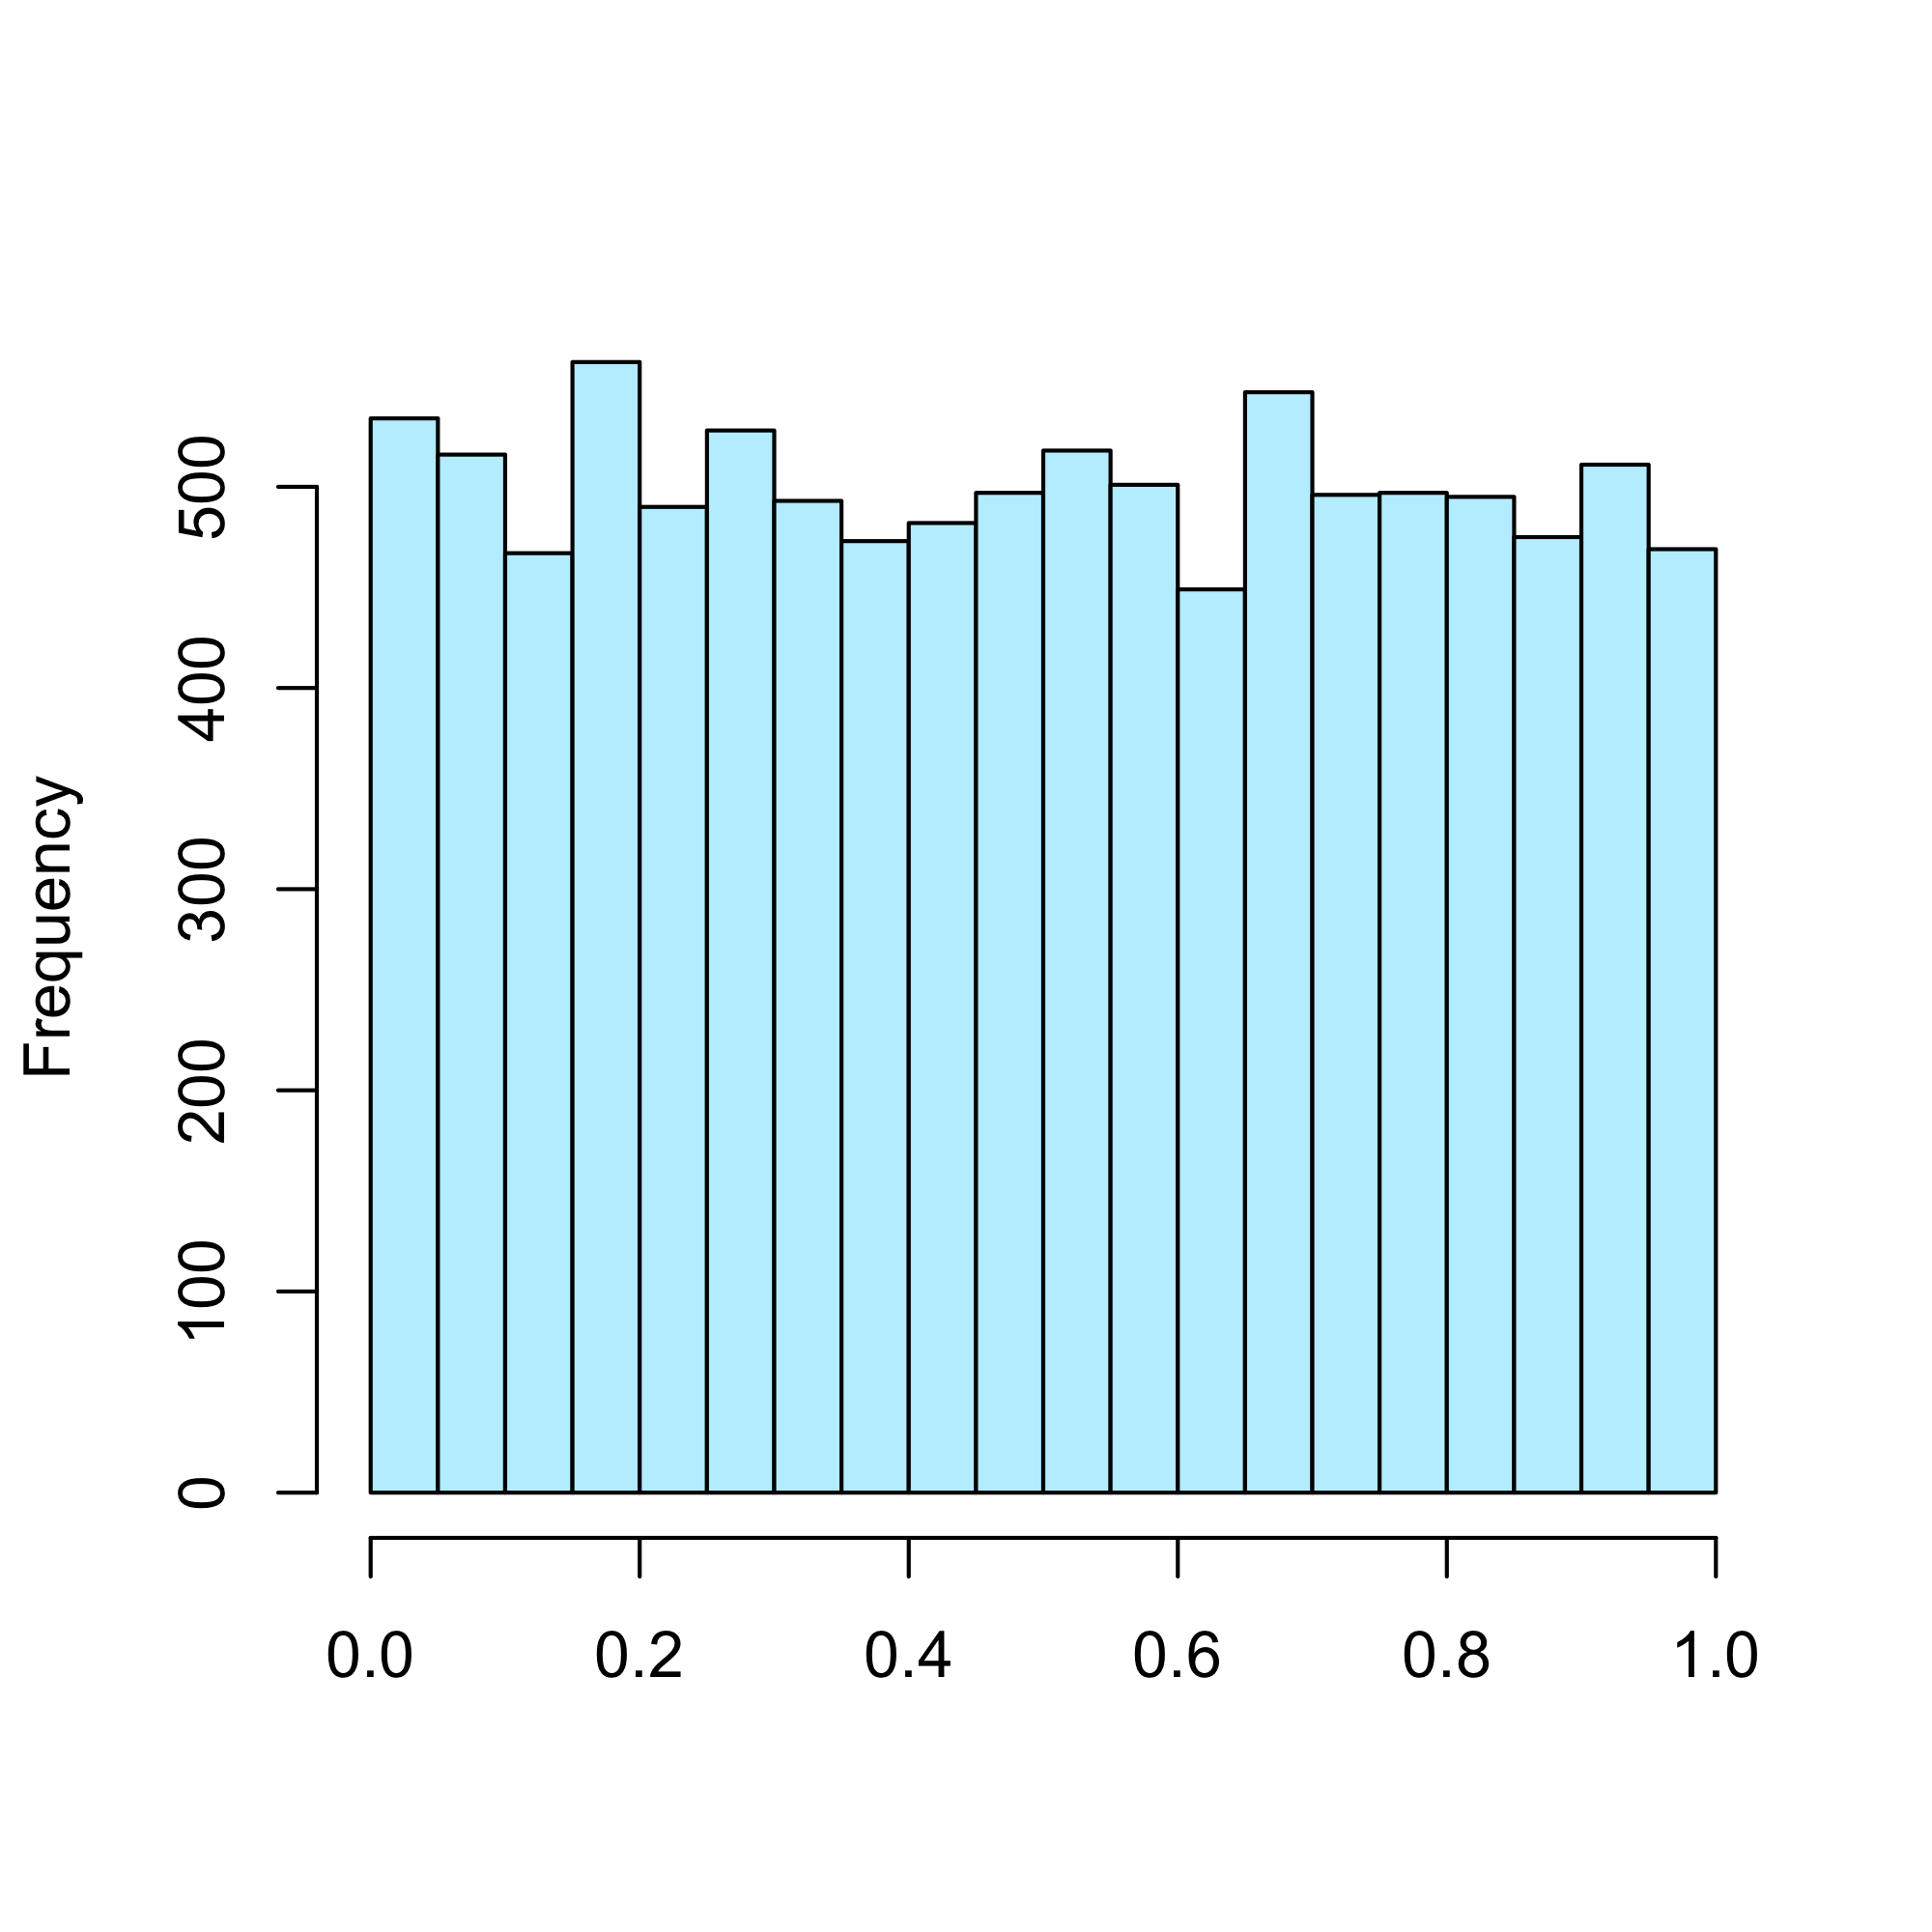
\includegraphics[width=\linewidth]{unif_acorn_hist.png}
		\caption{Histogram of one \textsc{ACORN} sample.}
		\label{fig:unif_acorn_hist}
	\end{subfigure}
	\begin{subfigure}[b]{0.45\linewidth}
		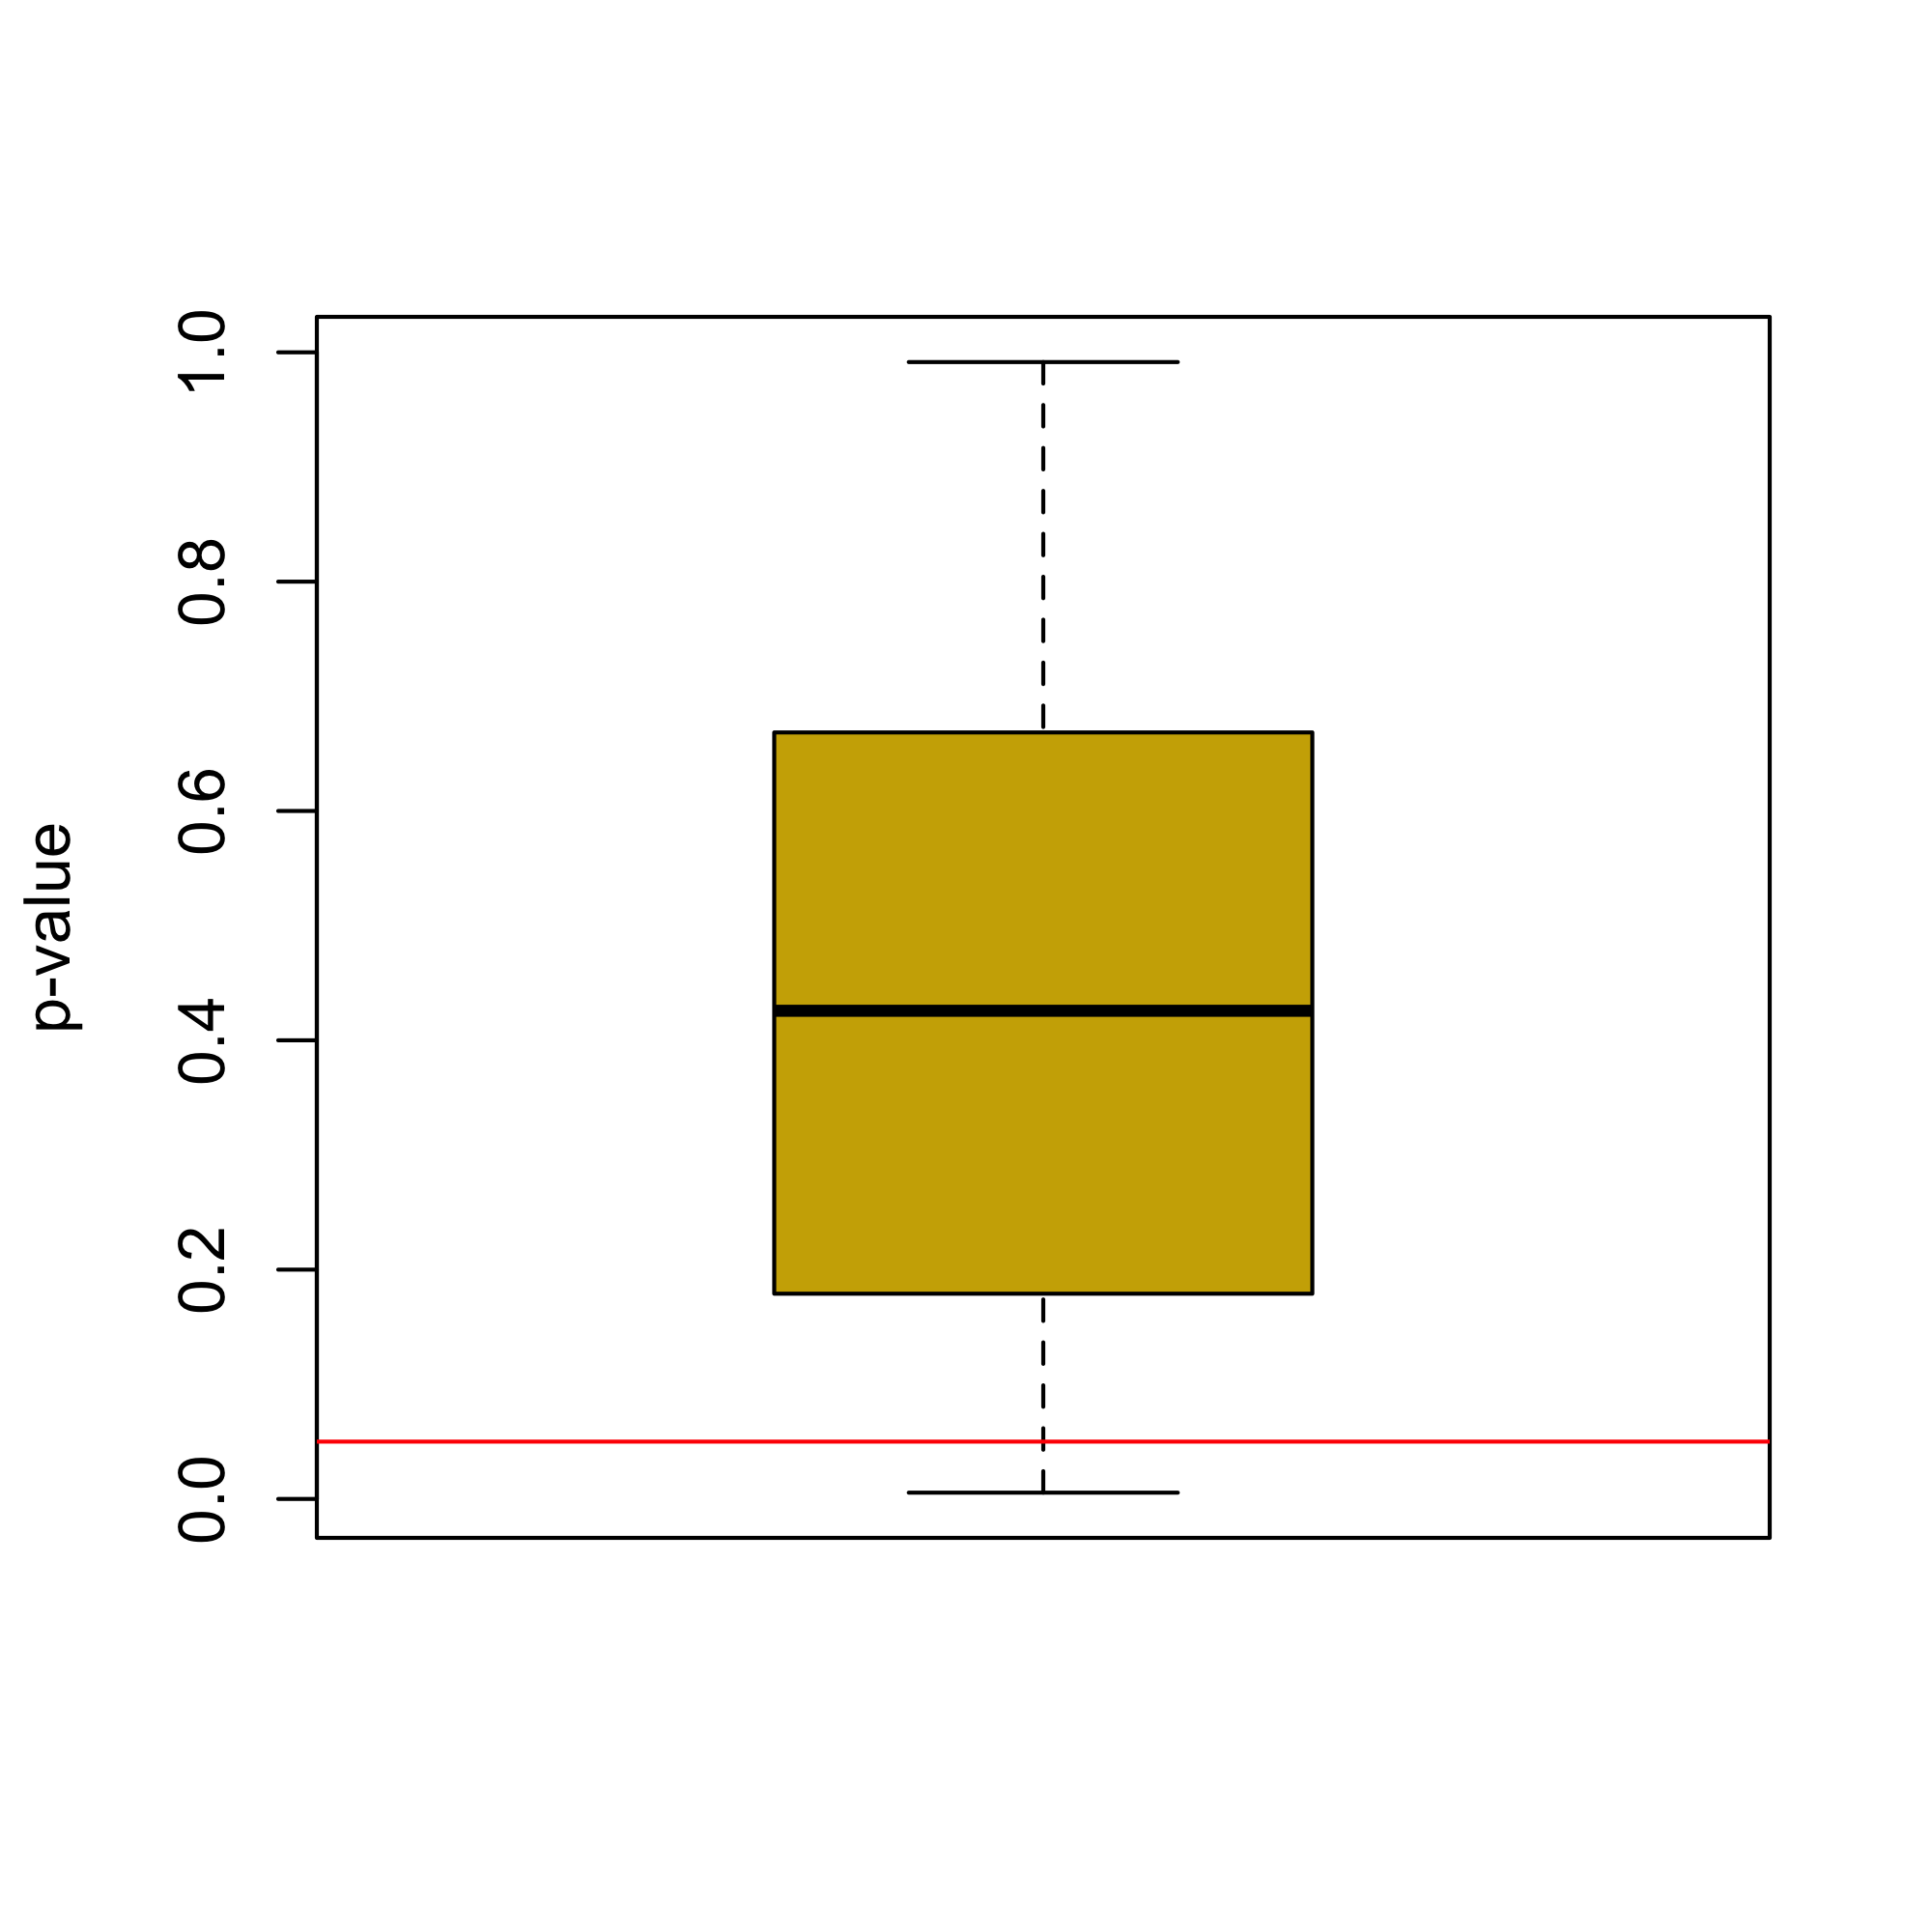
\includegraphics[width=\linewidth]{boxplot_pvalues_acorn.png}
		\caption{Boxplot of the $p$-values of a hundred \textsc{ACORN} samples.}
		\label{fig:boxplot_pvalues_acorn}
	\end{subfigure}
	\caption{\textsc{ACORN} generated numbers.} 
	\label{fig:acorn}
\end{figure}

\begin{algorithm}
	\caption{Additive Congruential Random Number Generator}
	\begin{flushleft}
		\textbf{Input: } Positive integers \texttt{M, n, y11, y12, $\dots$, y1k}.
		\\ \textbf{Output: } Array of \texttt{n} numbers with $\mathrm{Unif}$(0,1) distribution.
	\end{flushleft}
	
	\begin{algorithmic}[1]
		\State Create \texttt{n $\times$ k} matrix \texttt{A} with first row equal to \texttt{y11, y12, $\dots$, y1k}
		\For{\texttt{row} $=2, 3, \dots,$ \texttt{n} }
			\For{\texttt{col} $= 1, 2, \dots $ \texttt{k}}
				\If{\texttt{col} == 1}
					\State \texttt{A}[\texttt{row}][\texttt{col}] = \texttt{A}[\texttt{row-1}][\texttt{col}]
				\Else
					\State \texttt{x} = \texttt{A}[\texttt{row}][\texttt{col-1}] + \texttt{A}[\texttt{row-1}][\texttt{col}]	
					\State \texttt{A}[\texttt{row}][\texttt{col}] = \texttt{x mod M}
				\EndIf
			\EndFor
		\EndFor
		
		\State Make vector \texttt{numbers} equal to the \texttt{k}-th column of  \texttt{A}
		\State \Return \texttt{numbers / M}
	\end{algorithmic}
	\label{algo:acorn}
\end{algorithm}

\section{Methods for the normal distribution}
Methods for generating normal-distributed pseudo random numbers are shown next. First, the Box-Muller method and its polar form variation are presented. The sensitivity of Box-Muller method is explored. Finally, an algorithm based on the rejection method \cite{Ross_2006} is given. 

\subsection{Box-Muller method}
Algorithm \ref{algo:gaussian} presents the Box-muller method for sampling a pair $z_0, z_1$ of normal distributed pseudo-random numbers. A proof of why the algorithm works is given by Ross \cite{Ross_2000}. The algorithm was used to generate one-hundred samples of five-thousand normally distributed values, where the $p$-values resulting of performing the Shapiro Test on each sample was stored. This was compared to the $p$-values of R's \texttt{rnorm} method, and to variations of the Box-Muller method were only the first ($z_0$) or second ($z_1$) values sampled are kept. The comparison of these $p$-values is shown in Figure \ref{fig:pvalues_gaussian}. A summary is also shown in Table \ref{tab:pvalues_gaussian}.

\begin{table}
	\centering
	\caption{Number of $p$-values smaller and larger than 0.05 for different normal samples}
	\begin{tabular}{l r r r}
		\hline
		 Method &Less than 0.05 & Greater than 0.05 \\ 
		\hline
		Box-Muller, keeping only $z_0$ & 3 & 97 \\ 
		Box-Muller, keeping only $z_1$ &  6 & 94 \\ 
		Box-Muller, keeping both $z_0, z_1$ &  7 & 93 \\
		Using \texttt{rnorm} & 4 & 96 \\
		\hline
	\end{tabular}
	\label{tab:pvalues_gaussian}
\end{table}

\begin{algorithm}
	\caption{Box-Muller}
	\begin{flushleft}
		\textbf{Input: } Real numbers \texttt{mu, sigma}.
		\\ \textbf{Output: } Number with $\mathrm{Normal}$(\texttt{mu, sigma}) distribution.
	\end{flushleft}
	
	\begin{algorithmic}[1]
		\State Generate numbers \texttt{u1, u2} $\sim \mathrm{Unif}(0,1)$
		\State Make \texttt{z0 = sqrt(-2 $\ast$ log(u1)) $\ast$ cos (2 $\ast$ pi $\ast$ u2)} 
		\State Make \texttt{z1 = sqrt(-2 $\ast$ log(u1)) $\ast$ sin (2 $\ast$ pi $\ast$ u2)} 
		\State \Return \texttt{sigma} $\ast$ \texttt{z0 + mu}, \texttt{sigma} $\ast$ \texttt{z1 + mu}
	\end{algorithmic}
	\label{algo:gaussian}
\end{algorithm}

\begin{figure}
\centering
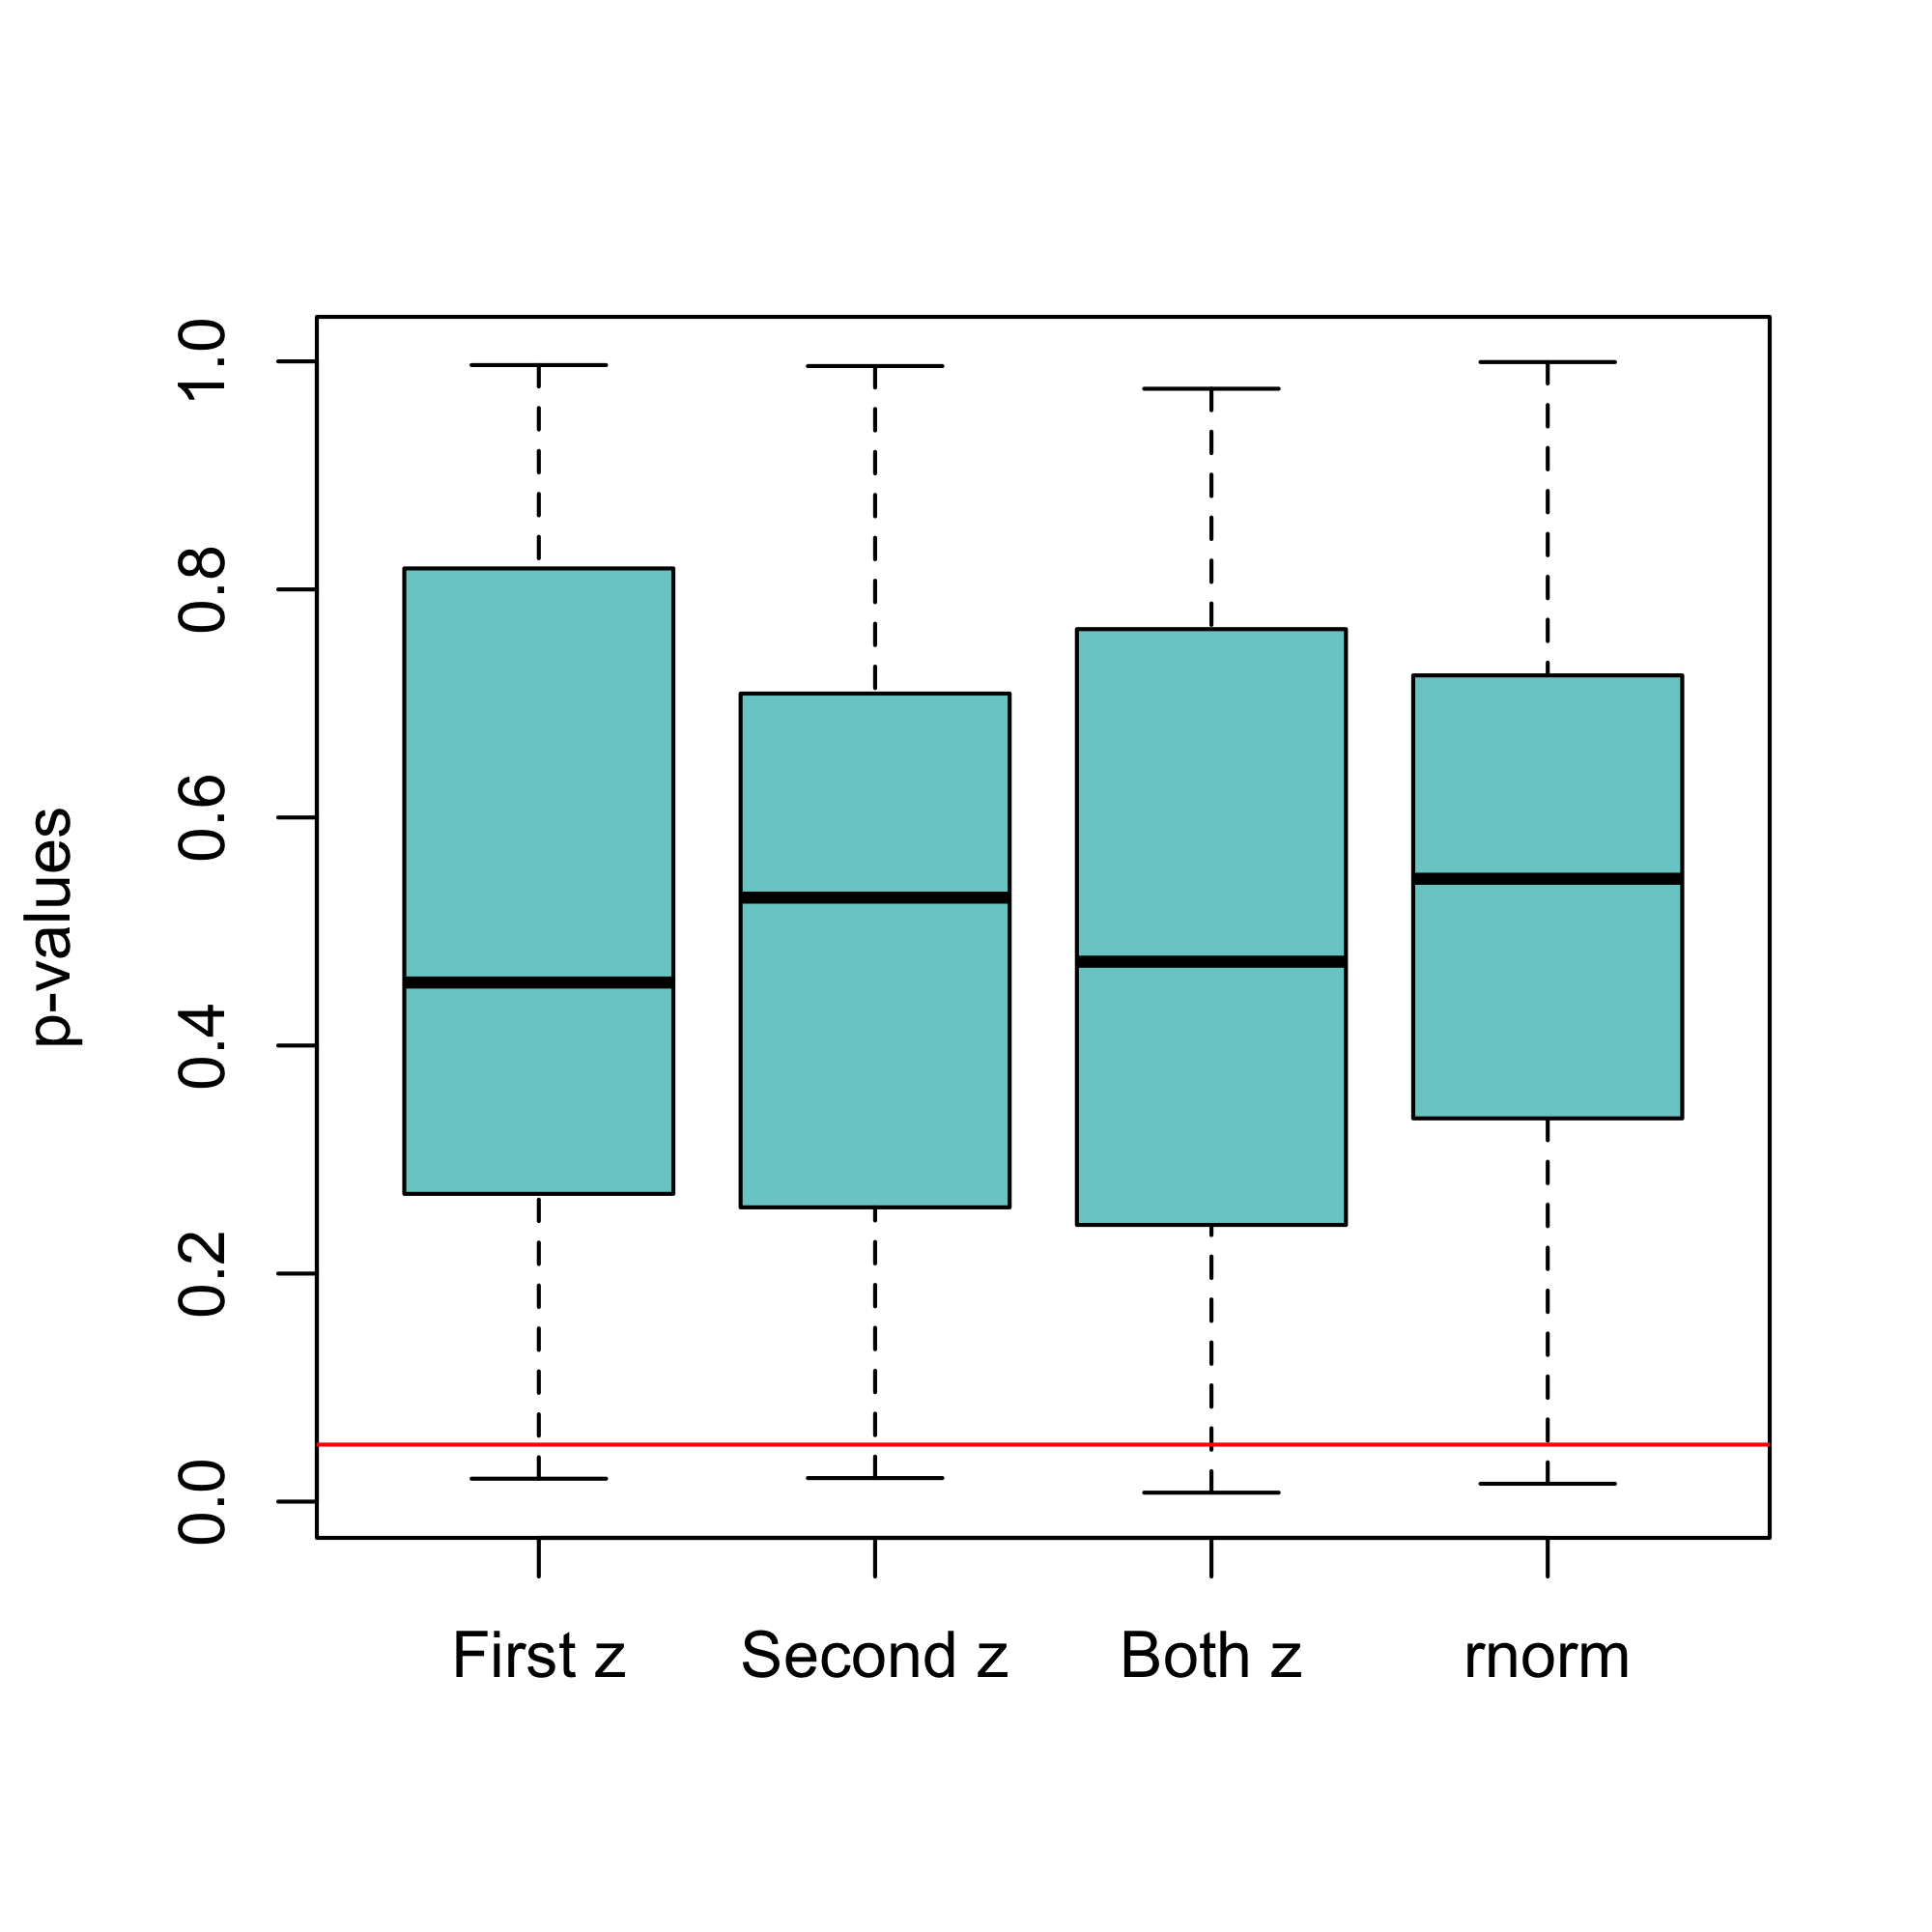
\includegraphics[width=.5\linewidth]{various_normal_pvalues}	
\caption{$p$-values obtained with different methods. Red line represents 0.05}
\label{fig:pvalues_gaussian}
\end{figure}

Next, to study the sensitivity of Algorithm \ref{algo:gaussian}, some variations were performed: first, instead of using R's \texttt{runif} to generate the uniform numbers, Algorithm \ref{algo:lgc} (\textsc{LGC}) was used instead. The other two variations consisted of using two \textit{non-independent} uniform distributed numbers. The first one uses $u_1 \sim \mathrm{Unif}(0,1)$ and  $u_2 = \frac{u_1}{2}$, while the second one uses $u_1 \sim \mathrm{Unif}(0,1)$ and  $u_2 = \frac{u_1 + 1}{2}$. As before, we generated a hundred samples and stored the $p$-values from Shapiro's Test. The results are summarized in Table \ref{tab:pvalues_gaussian_variations}.

\begin{table}
	\centering
	\caption{Number of $p$-values smaller and larger than 0.05 for different Normal samples}
	\begin{tabular}{l r r r}
		\hline
		Method &Less than 0.05 & Greater than 0.05 \\ 
		\hline
		Box-Muller, using \textsc{LGC}  & 8 & 92 \\ 
		Box-Muller, non-independent uniform values ($u_1 \sim \mathrm{Unif}(0,1)$ and  $u_2 = \frac{u_1}{2}$) &  100 & 0 \\ 
		Box-Muller, non-independent uniform values ($u_1 \sim \mathrm{Unif}(0,1)$ and  $u_2 = \frac{u_1 + 1}{2}$) &  100 & 0 \\
		\hline
	\end{tabular}
	\label{tab:pvalues_gaussian_variations}
\end{table}

It is observed that using a different method for generating the uniform pseudo-random numbers did not have much effect on the output. Using non-independent uniform numbers, however, made caused all samples to fail Shapiro's test.

\subsubsection{Box-Muller polar form}
A known variation of the Box-Muller method \cite{Ross_2000} is given in Algorithm \ref{algo:polar}. It works with the same principle, but avoids the computation of trigonometric functions. The performance of both Box-Muller forms was compared, concluding that Algorithm \ref{algo:polar} performs slower than Algorithm \ref{algo:gaussian}  77\% of the time, with an average difference of 0.001 seconds. 

\begin{algorithm}
	\caption{Box-Muller Transform. Polar version}
	\begin{flushleft}
		\textbf{Input: } Real numbers \texttt{mu, sigma}.
		\\ \textbf{Output: } Number with $\mathrm{Normal}$(\texttt{mu, sigma}) distribution.
	\end{flushleft}
	
	\begin{algorithmic}[1]
		\Repeat
		\State Generate numbers \texttt{u1, u2} $\sim \mathrm{Unif}(0,1)$
		\State Make \texttt{V1 = 2 $\ast$ u1 - 1}
		\State Make \texttt{V2 = 2 $\ast$ u2 - 1}
		\State Make \texttt{S = V1$^2$ + V2$^2$}
		\Until{\texttt{S} $\leq$ 1}
		\State Make \texttt{Z1 = sqrt( (-2 $\ast$ log(S) ) / S ) $\ast$ V1}
		\State Make \texttt{Z2 = sqrt( (-2 $\ast$ log(S) ) / S ) $\ast$ V2} 
		\State \Return \texttt{sigma} $\ast$ \texttt{Z1 + mu}, \texttt{sigma} $\ast$ \texttt{Z2 + mu}
	\end{algorithmic}
	\label{algo:polar}
\end{algorithm}

\subsection{Rejection method}
Algorithm \ref{algo:rejection} is based on the Rejection Method, and is explained in Ross' Simulation book \cite{Ross_2006}.  As in previous sections, a hundred samples were generated using Algorithm \ref{algo:rejection} and the $p$-values of this samples under Shapiro's test were stored, as can be seen in Figure \ref{fig:pvalues_rejection}. A histogram of a five-thousand sample generated with Algorithm \ref{algo:rejection} is shown in Figure \ref{fig:rejection_hist}, next to a histogram of five-thousand numbers generated by R's \texttt{rnorm} in Figure \ref{fig:rnorm_hist}.

\begin{figure}
	\centering
	\begin{subfigure}[b]{0.45\linewidth}
		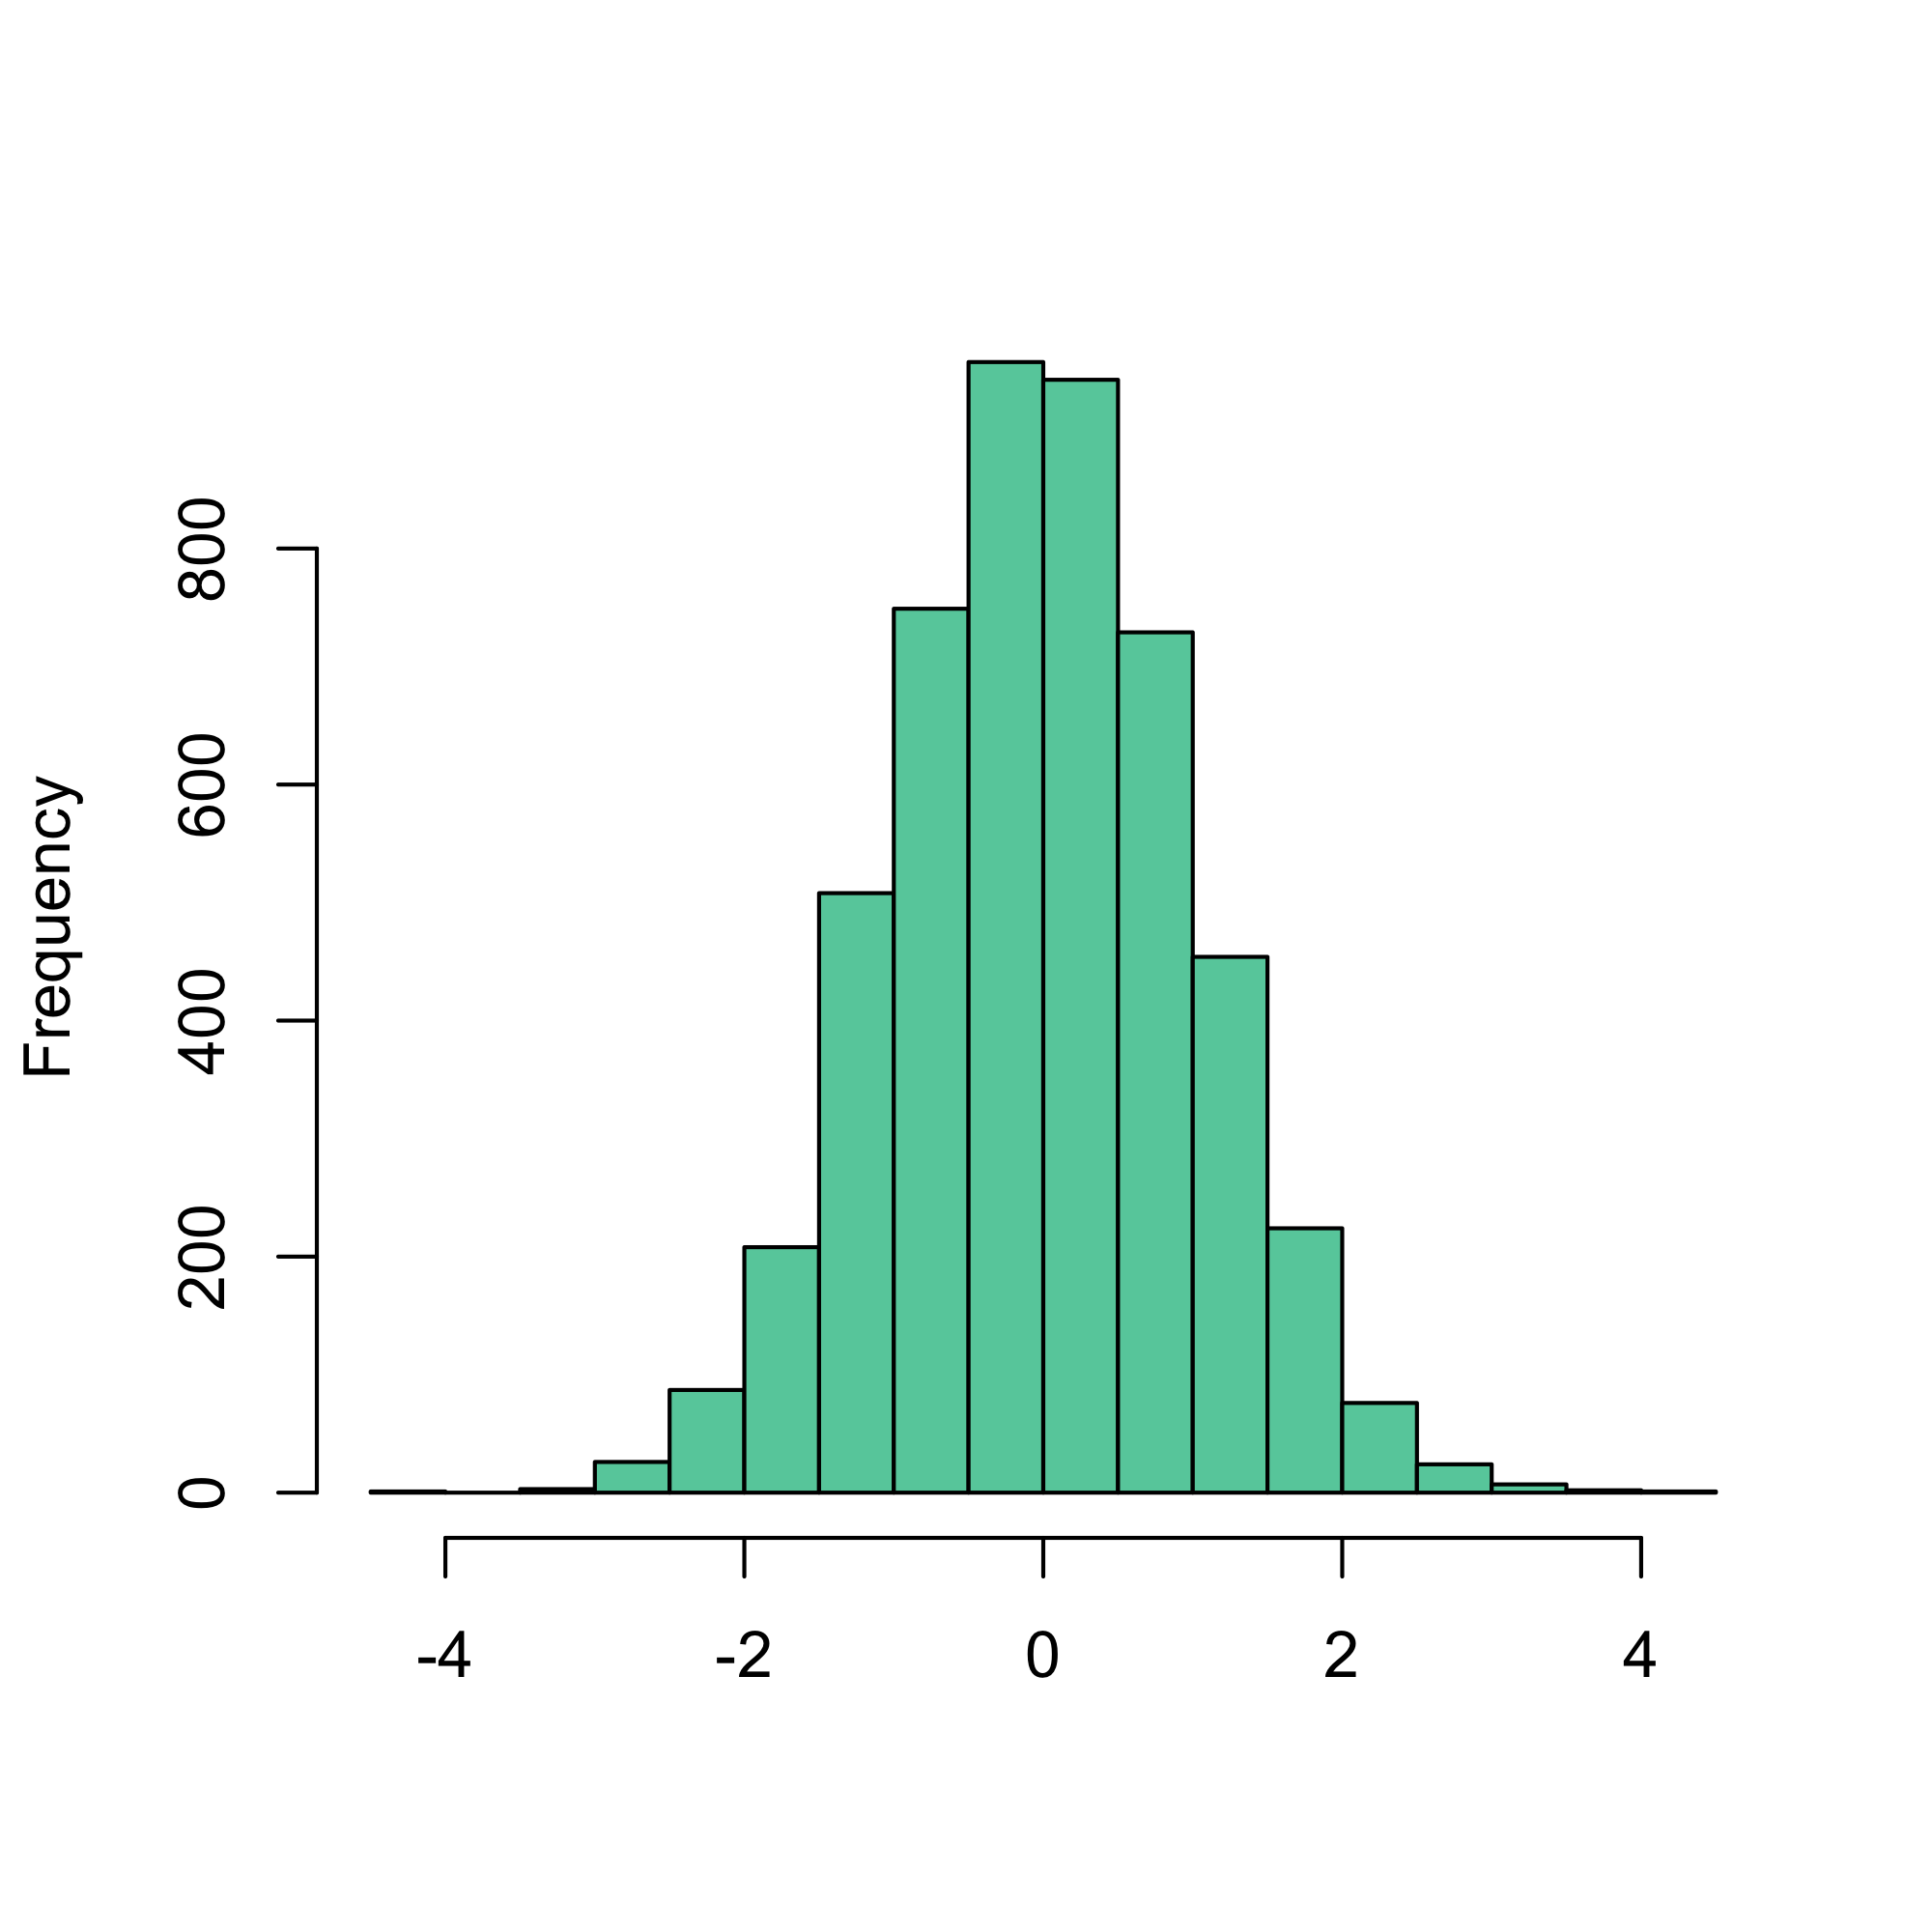
\includegraphics[width=\linewidth]{hist_rm_normal.png}
		\caption{Histogram of one five-thousand number sample given by Algorithm \ref{algo:rejection}.}
		\label{fig:rejection_hist}
	\end{subfigure}
	\begin{subfigure}[b]{0.45\linewidth}
		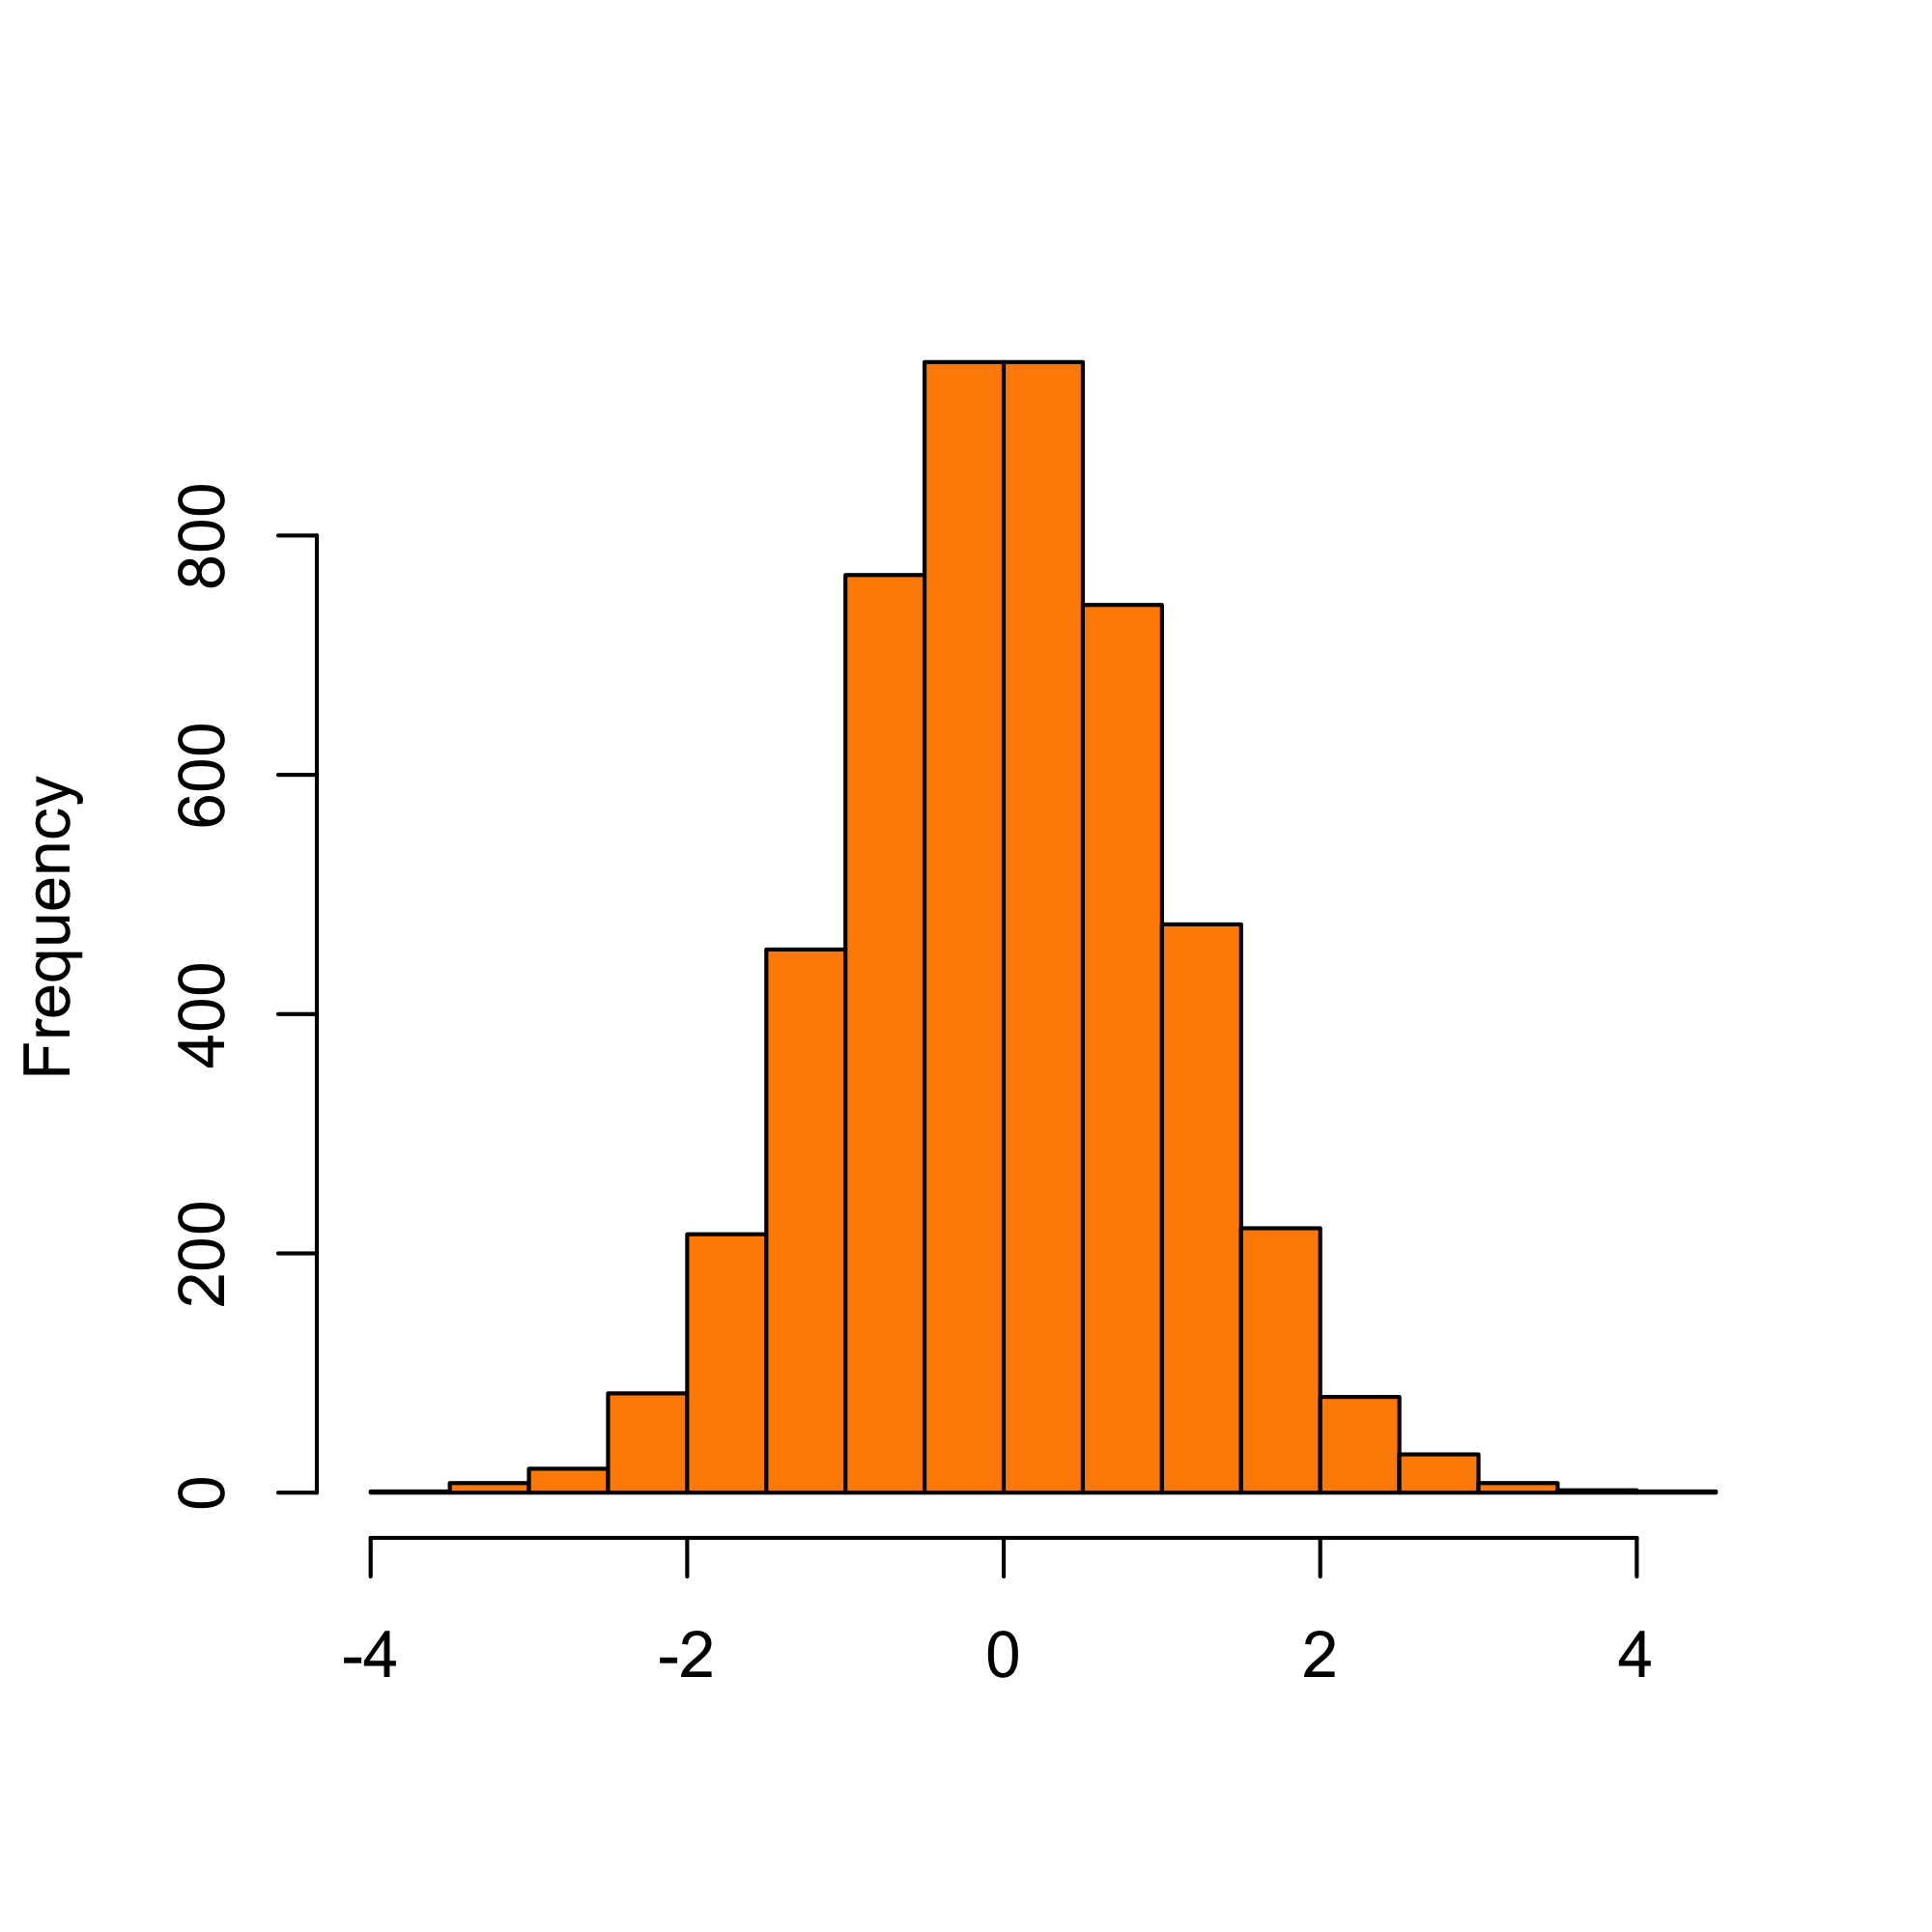
\includegraphics[width=\linewidth]{hist_rnorm.png}
		\caption{Histogram of one five-thousand number sample given by \texttt{rnorm}.}
		\label{fig:rnorm_hist}
	\end{subfigure}
	\begin{subfigure}[b]{0.45\linewidth}
	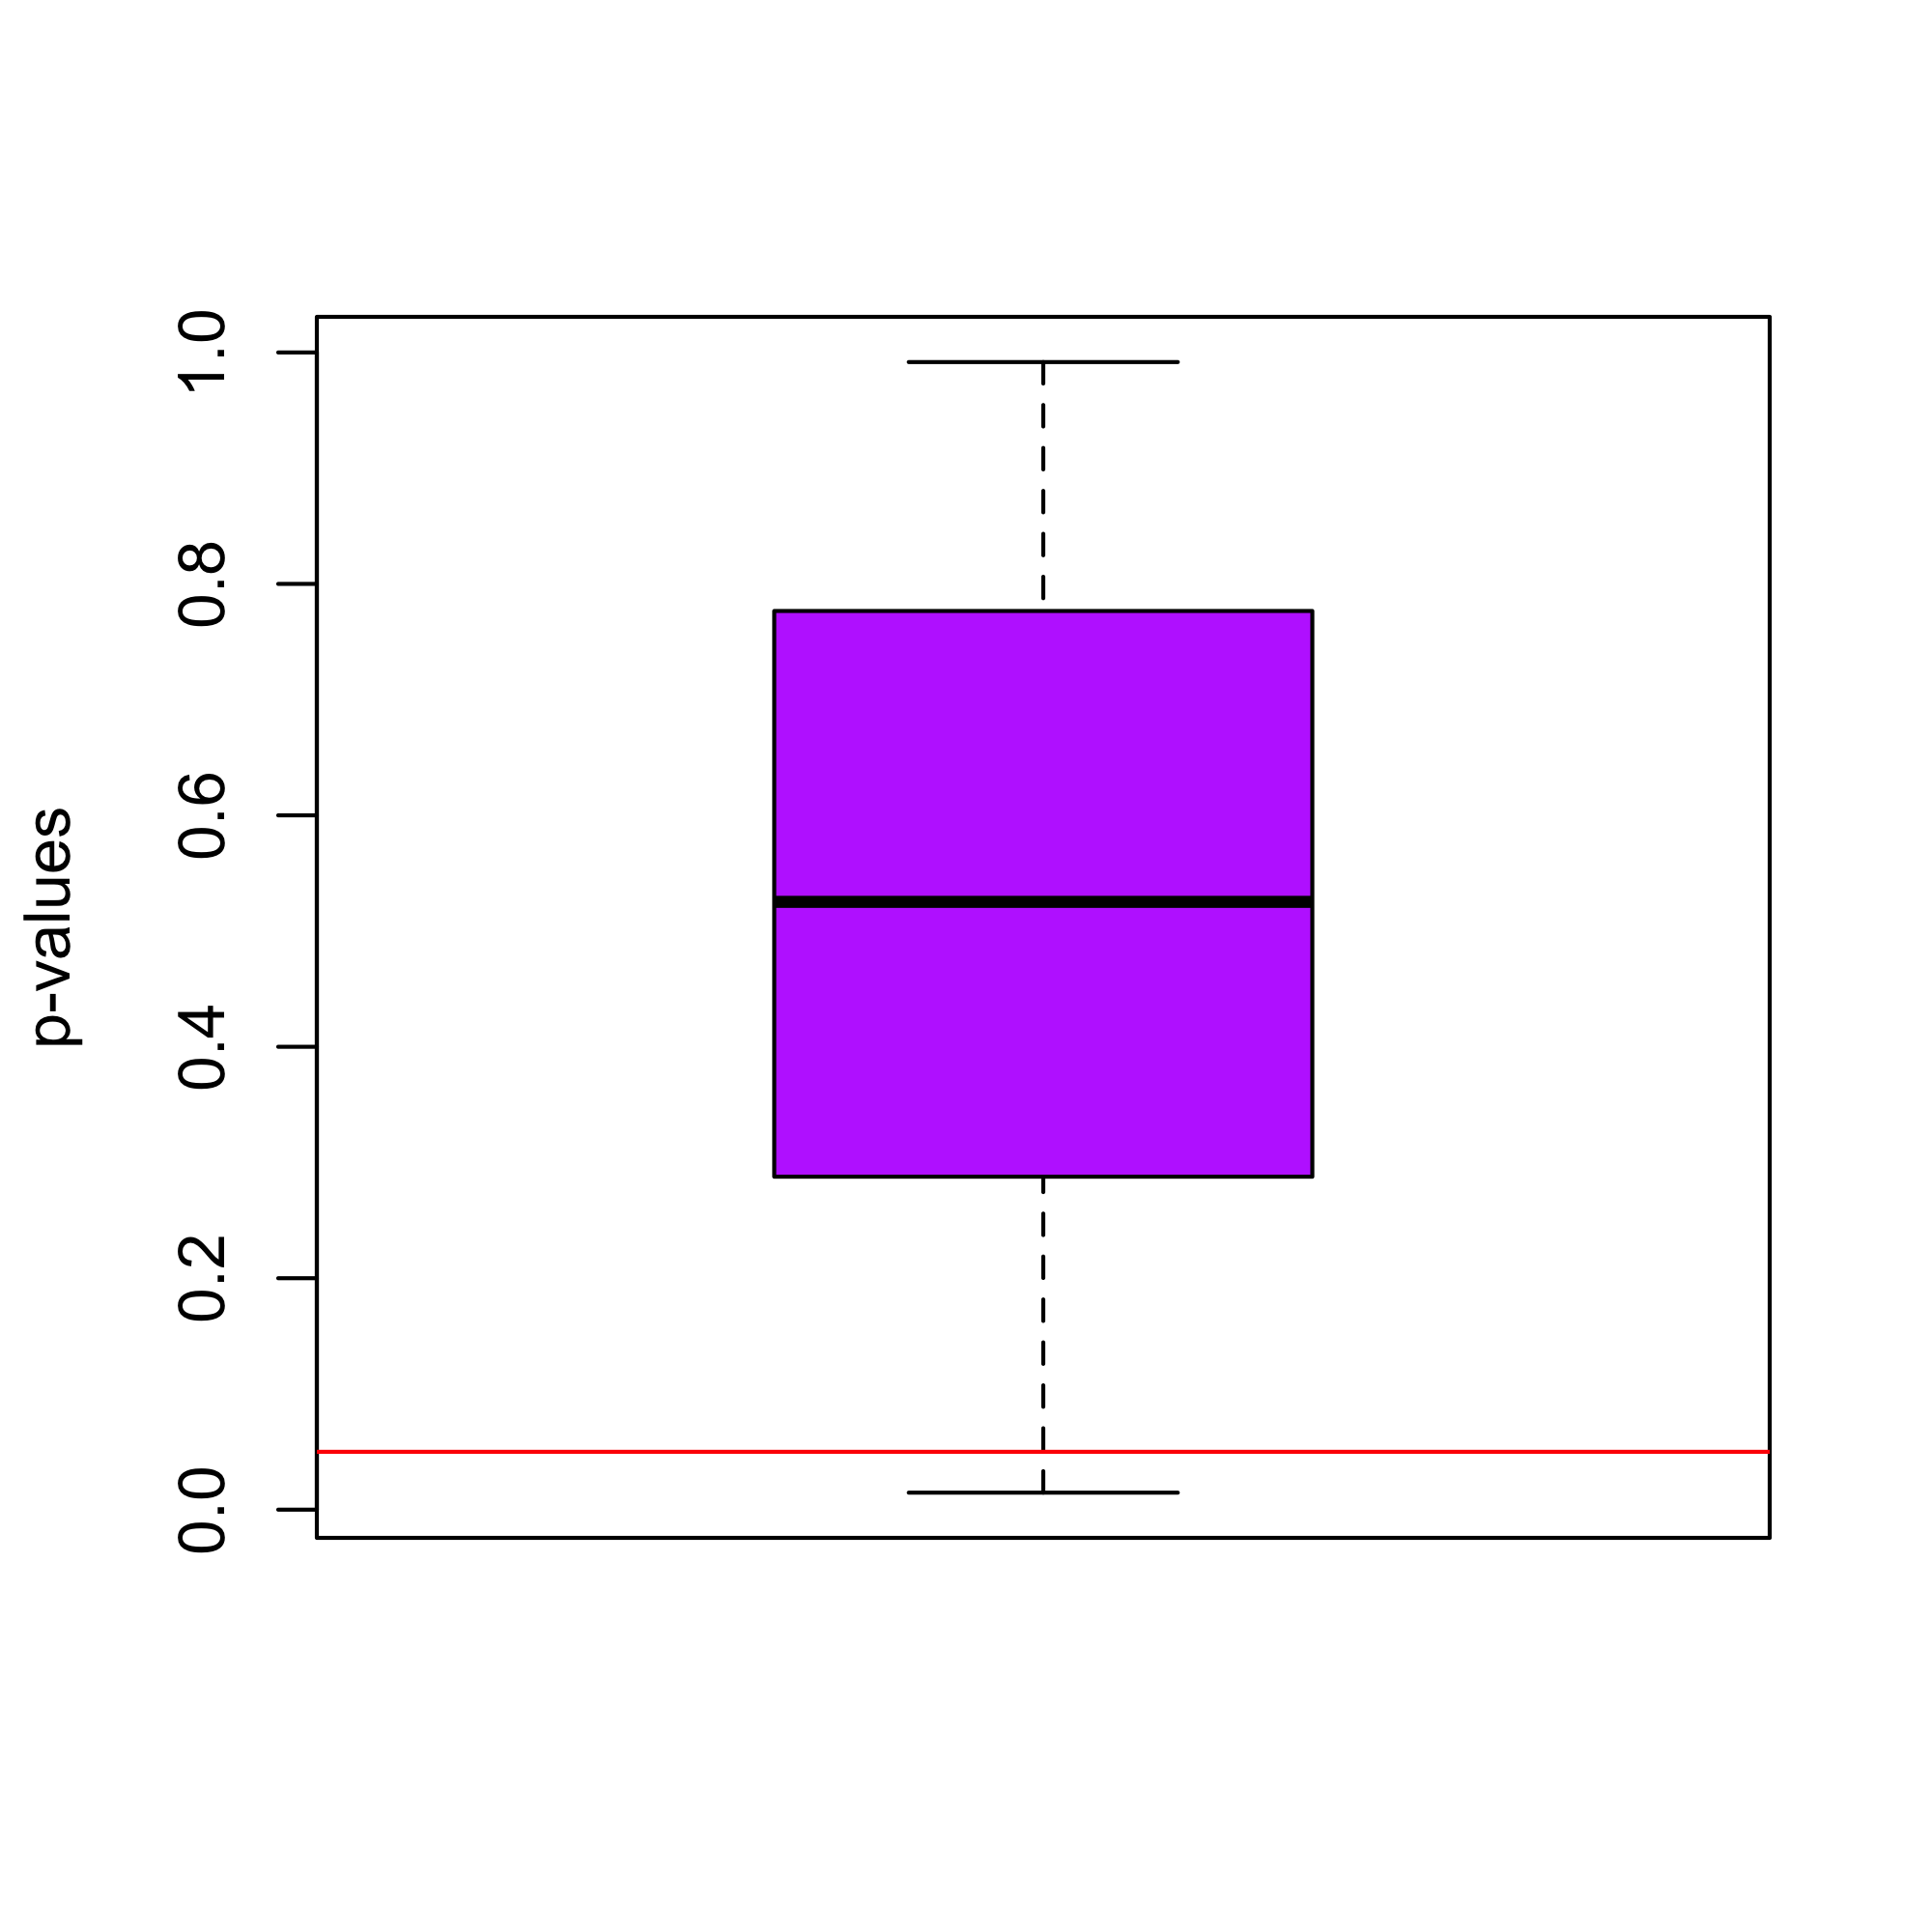
\includegraphics[width=\linewidth]{pvalues_rm_normal.png}
	\caption{Boxplot of the $p$-values of a hundred samples given by Algorithm \ref{algo:rejection}.}
	\label{fig:pvalues_rejection}
	\end{subfigure}
	\caption{Comparing Algorithm \ref{algo:rejection} to \texttt{rnorm}. } 
	\label{fig:rejection_method}
\end{figure}


\begin{algorithm}
	\caption{Rejection method. Normal distribution}
	\begin{flushleft}
		\textbf{Input: } Real numbers \texttt{mu, sigma}.
		\\ \textbf{Output: } Number with $\mathrm{Normal}$(\texttt{mu, sigma}) distribution.
	\end{flushleft}
	
	\begin{algorithmic}[1]
		\State Generate \texttt{y1, y2} $\sim \mathrm{Exp}(1)$
		\While{ \texttt{y2 - (y1-1)$^2$ / 2 $<$ 0} }
			\State Generate \texttt{y1, y2} $\sim \mathrm{Exp}(1)$
		\EndWhile
		\State Generate \texttt{u} $\sim \mathrm{Unif}(0,1)$
		\If{ \texttt{u} $\leq 1/2$}
			\State Make \texttt{z = y1}
		\Else 
			\State Make \texttt{z = - y1}
		\EndIf
		\State \Return \texttt{sigma $\ast$ z + mu}
	\end{algorithmic}
	\label{algo:rejection}
\end{algorithm}


\section{Conclusions}
It is observed how methods for different generating non-uniform pseudo-random numbers commonly rely on the generation of uniform distributed pseudo-random numbers. The \textsc{LGC} and \textsc{ACORN} methods both seem to give good results, even when used with methods like Box-Muller's. Further study should include pseudo-random number generators for different distributions. Given how Frosini's and Shapiro's test are both distribution dependent (uniform, normal), the study of generators for new distributions should be accompanied with the study of new statistical tests.

\section{Acknowledgments}
We thank Professor Elisa Schaeffer for providing code for the Box-Muller method in Algorithm \ref{algo:gaussian} and the Linear Congruential Generator in Algorithm \ref{algo:lgc}.


%%%%%%%%%%%%%%%%%%%%%%%%%%%%

\bibliographystyle{siam}
\bibliography{refr}


%%%%%%%%%%%%%%%%%%%%%%%%%%%%
\end{document}
